\documentclass[14pt]{extbook}
\usepackage{multicol, enumerate, enumitem, hyperref, color, soul, setspace, parskip, fancyhdr} %General Packages
\usepackage{amssymb, amsthm, amsmath, bbm, latexsym, units, mathtools} %Math Packages
\everymath{\displaystyle} %All math in Display Style
% Packages with additional options
\usepackage[headsep=0.5cm,headheight=12pt, left=1 in,right= 1 in,top= 1 in,bottom= 1 in]{geometry}
\usepackage[usenames,dvipsnames]{xcolor}
\usepackage{dashrule}  % Package to use the command below to create lines between items
\newcommand{\litem}[1]{\item#1\hspace*{-1cm}\rule{\textwidth}{0.4pt}}
\pagestyle{fancy}
\lhead{Makeup Progress Quiz 3}
\chead{}
\rhead{Version B}
\lfoot{4315-3397}
\cfoot{}
\rfoot{Fall 2020}
\begin{document}

\begin{enumerate}
\litem{
Choose the equation of the function graphed below.
\begin{center}
    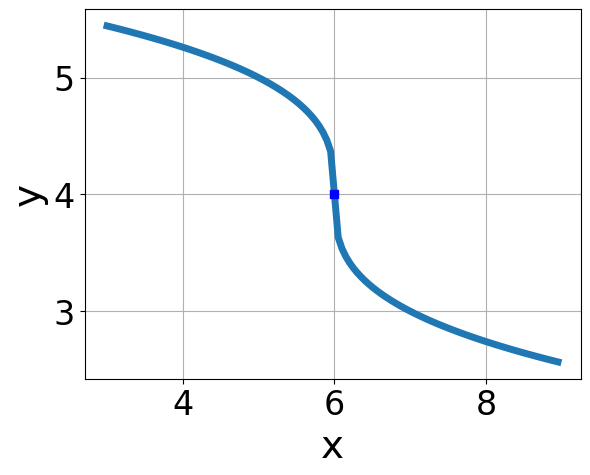
\includegraphics[width=0.5\textwidth]{../Figures/radicalGraphToEquationCopyB.png}
\end{center}
\begin{enumerate}[label=\Alph*.]
\item \( f(x) = - \sqrt[3]{x - 6} + 4 \)
\item \( f(x) = \sqrt[3]{x - 6} + 4 \)
\item \( f(x) = - \sqrt[3]{x + 6} + 4 \)
\item \( f(x) = \sqrt[3]{x + 6} + 4 \)
\item \( \text{None of the above} \)

\end{enumerate} }
\litem{
What is the domain of the function below?\[ f(x) = \sqrt[5]{-4 x + 5} \]\begin{enumerate}[label=\Alph*.]
\item \( \text{The domain is } (-\infty, a], \text{   where } a \in [0.91, 1.3] \)
\item \( \text{The domain is } [a, \infty), \text{   where } a \in [0.75, 1.12] \)
\item \( \text{The domain is } (-\infty, a], \text{   where } a \in [0.25, 1.12] \)
\item \( \text{The domain is } [a, \infty), \text{   where } a \in [1.12, 1.93] \)
\item \( (-\infty, \infty) \)

\end{enumerate} }
\litem{
Solve the radical equation below. Then, choose the interval(s) that the solution(s) belongs to.\[ \sqrt{-7 x - 2} - \sqrt{-8 x - 3} = 0 \]\begin{enumerate}[label=\Alph*.]
\item \( x \in [-1.9,-0.8] \)
\item \( x_1 \in [-1.9, -0.8] \text{ and } x_2 \in [-1.29,2.71] \)
\item \( \text{All solutions lead to invalid or complex values in the equation.} \)
\item \( x \in [3.9,5.3] \)
\item \( x_1 \in [-0.5, 0.3] \text{ and } x_2 \in [-1.29,2.71] \)

\end{enumerate} }
\litem{
Choose the graph of the equation below.\[ f(x) = \sqrt[3]{x + 14} + 6 \]\begin{enumerate}[label=\Alph*.]
\begin{multicols}{2}\item 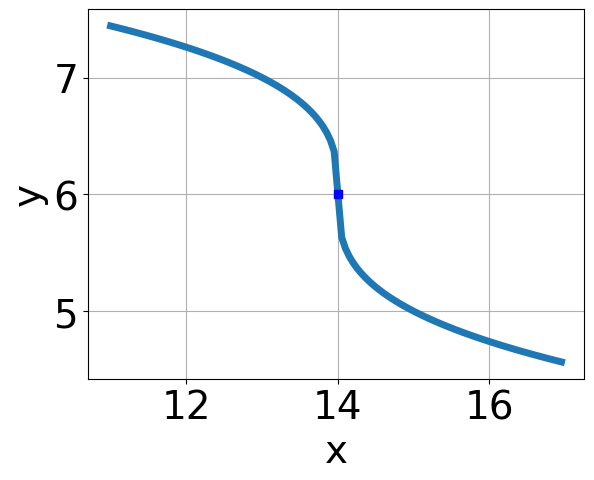
\includegraphics[width = 0.3\textwidth]{../Figures/radicalEquationToGraphAB.png}\item 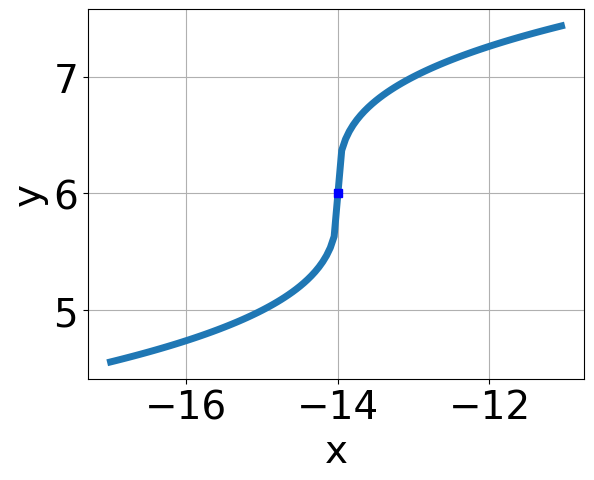
\includegraphics[width = 0.3\textwidth]{../Figures/radicalEquationToGraphBB.png}\item 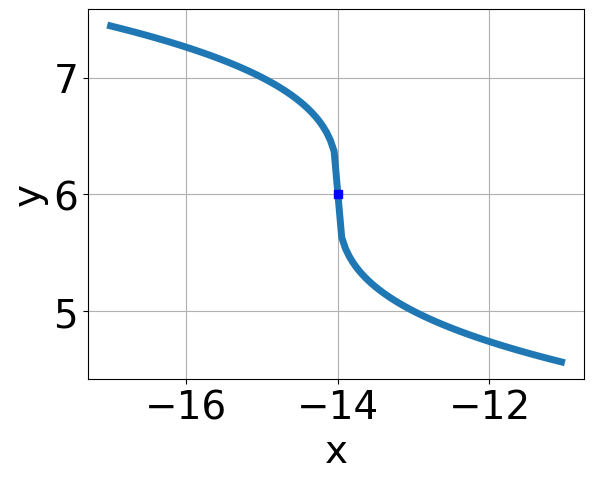
\includegraphics[width = 0.3\textwidth]{../Figures/radicalEquationToGraphCB.png}\item 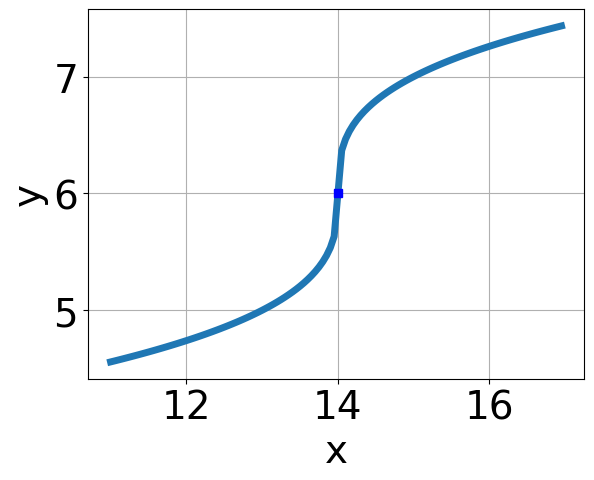
\includegraphics[width = 0.3\textwidth]{../Figures/radicalEquationToGraphDB.png}\end{multicols}\item None of the above.
\end{enumerate} }
\litem{
What is the domain of the function below?\[ f(x) = \sqrt[5]{-3 x + 5} \]\begin{enumerate}[label=\Alph*.]
\item \( \text{The domain is } [a, \infty), \text{   where } a \in [1.24, 1.78] \)
\item \( \text{The domain is } [a, \infty), \text{   where } a \in [0.09, 1.13] \)
\item \( \text{The domain is } (-\infty, a], \text{   where } a \in [1.01, 2.21] \)
\item \( \text{The domain is } (-\infty, a], \text{   where } a \in [0.13, 1.06] \)
\item \( (-\infty, \infty) \)

\end{enumerate} }
\litem{
Choose the graph of the equation below.\[ f(x) = \sqrt{x - 14} + 3 \]\begin{enumerate}[label=\Alph*.]
\begin{multicols}{2}\item 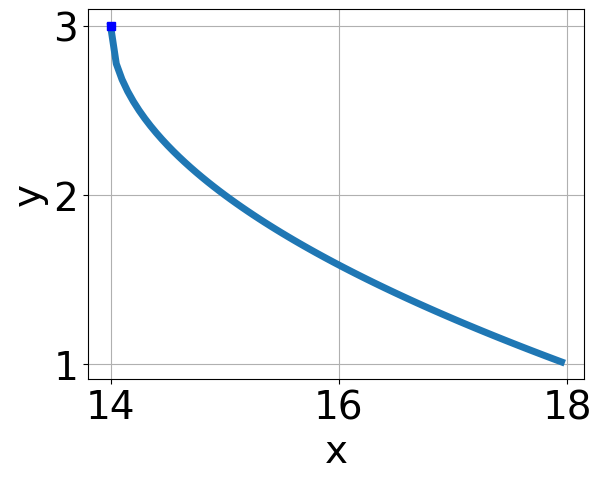
\includegraphics[width = 0.3\textwidth]{../Figures/radicalEquationToGraphCopyAB.png}\item 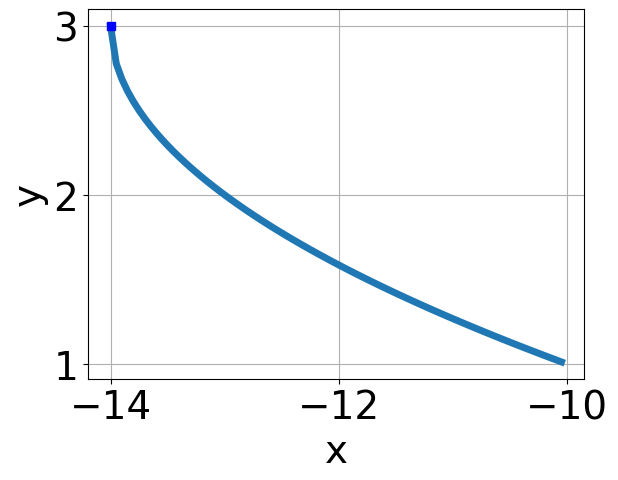
\includegraphics[width = 0.3\textwidth]{../Figures/radicalEquationToGraphCopyBB.png}\item 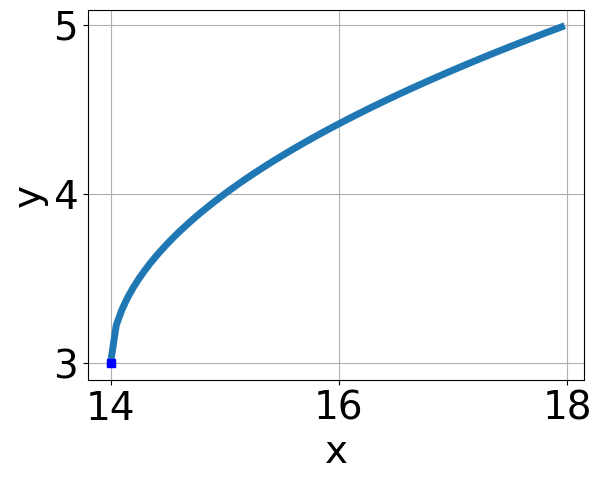
\includegraphics[width = 0.3\textwidth]{../Figures/radicalEquationToGraphCopyCB.png}\item 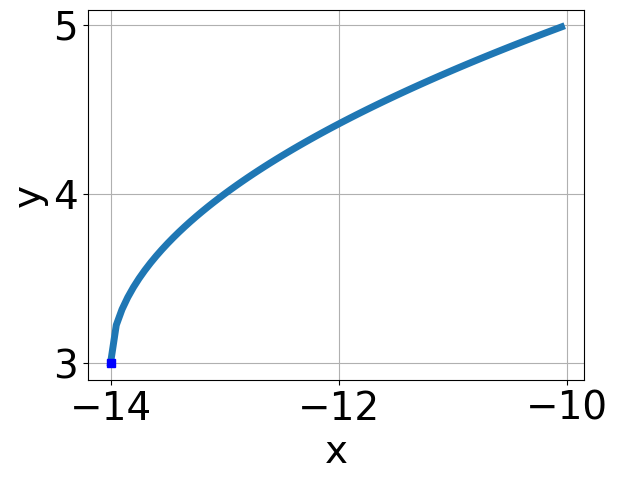
\includegraphics[width = 0.3\textwidth]{../Figures/radicalEquationToGraphCopyDB.png}\end{multicols}\item None of the above.
\end{enumerate} }
\litem{
Solve the radical equation below. Then, choose the interval(s) that the solution(s) belongs to.\[ \sqrt{-32 x^2 - 63} - \sqrt{100 x} = 0 \]\begin{enumerate}[label=\Alph*.]
\item \( \text{All solutions lead to invalid or complex values in the equation.} \)
\item \( x_1 \in [-2.27, -1.5] \text{ and } x_2 \in [-5.88,0.12] \)
\item \( x \in [-2.27,-1.5] \)
\item \( x \in [-1.39,-0.84] \)
\item \( x_1 \in [2.01, 3.28] \text{ and } x_2 \in [-0.12,2.88] \)

\end{enumerate} }
\litem{
Solve the radical equation below. Then, choose the interval(s) that the solution(s) belongs to.\[ \sqrt{24 x^2 - 28} - \sqrt{-26 x} = 0 \]\begin{enumerate}[label=\Alph*.]
\item \( x_1 \in [-4.75, -0.75] \text{ and } x_2 \in [0.3,0.8] \)
\item \( x \in [-4.75,-0.75] \)
\item \( x_1 \in [-1.33, 2.67] \text{ and } x_2 \in [0.7,2.9] \)
\item \( x \in [-1.33,2.67] \)
\item \( \text{All solutions lead to invalid or complex values in the equation.} \)

\end{enumerate} }
\litem{
Solve the radical equation below. Then, choose the interval(s) that the solution(s) belongs to.\[ \sqrt{-6 x + 8} - \sqrt{-7 x - 7} = 0 \]\begin{enumerate}[label=\Alph*.]
\item \( \text{All solutions lead to invalid or complex values in the equation.} \)
\item \( x_1 \in [-5, 3] \text{ and } x_2 \in [0.33,3.33] \)
\item \( x \in [-17,-12] \)
\item \( x_1 \in [-17, -12] \text{ and } x_2 \in [0.33,3.33] \)
\item \( x \in [-5,3] \)

\end{enumerate} }
\litem{
Choose the equation of the function graphed below.
\begin{center}
    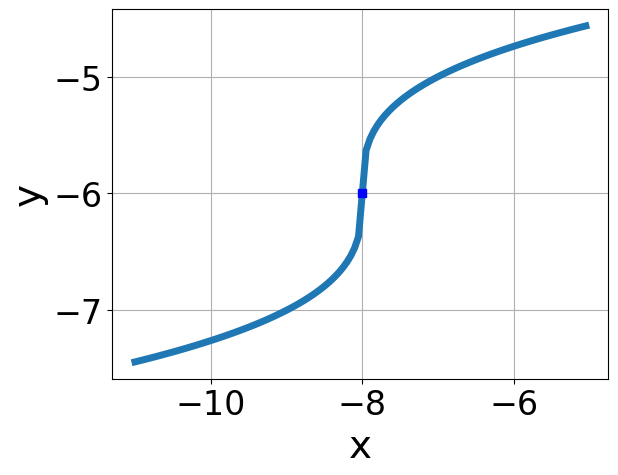
\includegraphics[width=0.5\textwidth]{../Figures/radicalGraphToEquationB.png}
\end{center}
\begin{enumerate}[label=\Alph*.]
\item \( f(x) = \sqrt{x - 8} - 6 \)
\item \( f(x) = - \sqrt{x + 8} - 6 \)
\item \( f(x) = \sqrt{x + 8} - 6 \)
\item \( f(x) = - \sqrt{x - 8} - 6 \)
\item \( \text{None of the above} \)

\end{enumerate} }
\end{enumerate}

\end{document}